\documentclass[1p]{elsarticle_modified}
%\bibliographystyle{elsarticle-num}

%\usepackage[colorlinks]{hyperref}
%\usepackage{abbrmath_seonhwa} %\Abb, \Ascr, \Acal ,\Abf, \Afrak
\usepackage{amsfonts}
\usepackage{amssymb}
\usepackage{amsmath}
\usepackage{amsthm}
\usepackage{scalefnt}
\usepackage{amsbsy}
\usepackage{kotex}
\usepackage{caption}
\usepackage{subfig}
\usepackage{color}
\usepackage{graphicx}
\usepackage{xcolor} %% white, black, red, green, blue, cyan, magenta, yellow
\usepackage{float}
\usepackage{setspace}
\usepackage{hyperref}

\usepackage{tikz}
\usetikzlibrary{arrows}

\usepackage{multirow}
\usepackage{array} % fixed length table
\usepackage{hhline}

%%%%%%%%%%%%%%%%%%%%%
\makeatletter
\renewcommand*\env@matrix[1][\arraystretch]{%
	\edef\arraystretch{#1}%
	\hskip -\arraycolsep
	\let\@ifnextchar\new@ifnextchar
	\array{*\c@MaxMatrixCols c}}
\makeatother %https://tex.stackexchange.com/questions/14071/how-can-i-increase-the-line-spacing-in-a-matrix
%%%%%%%%%%%%%%%

\usepackage[normalem]{ulem}

\newcommand{\msout}[1]{\ifmmode\text{\sout{\ensuremath{#1}}}\else\sout{#1}\fi}
%SOURCE: \msout is \stkout macro in https://tex.stackexchange.com/questions/20609/strikeout-in-math-mode

\newcommand{\cancel}[1]{
	\ifmmode
	{\color{red}\msout{#1}}
	\else
	{\color{red}\sout{#1}}
	\fi
}

\newcommand{\add}[1]{
	{\color{blue}\uwave{#1}}
}

\newcommand{\replace}[2]{
	\ifmmode
	{\color{red}\msout{#1}}{\color{blue}\uwave{#2}}
	\else
	{\color{red}\sout{#1}}{\color{blue}\uwave{#2}}
	\fi
}

\newcommand{\Sol}{\mathcal{S}} %segment
\newcommand{\D}{D} %diagram
\newcommand{\A}{\mathcal{A}} %arc


%%%%%%%%%%%%%%%%%%%%%%%%%%%%%5 test

\def\sl{\operatorname{\textup{SL}}(2,\Cbb)}
\def\psl{\operatorname{\textup{PSL}}(2,\Cbb)}
\def\quan{\mkern 1mu \triangleright \mkern 1mu}

\theoremstyle{definition}
\newtheorem{thm}{Theorem}[section]
\newtheorem{prop}[thm]{Proposition}
\newtheorem{lem}[thm]{Lemma}
\newtheorem{ques}[thm]{Question}
\newtheorem{cor}[thm]{Corollary}
\newtheorem{defn}[thm]{Definition}
\newtheorem{exam}[thm]{Example}
\newtheorem{rmk}[thm]{Remark}
\newtheorem{alg}[thm]{Algorithm}

\newcommand{\I}{\sqrt{-1}}
\begin{document}

%\begin{frontmatter}
%
%\title{Boundary parabolic representations of knots up to 8 crossings}
%
%%% Group authors per affiliation:
%\author{Yunhi Cho} 
%\address{Department of Mathematics, University of Seoul, Seoul, Korea}
%\ead{yhcho@uos.ac.kr}
%
%
%\author{Seonhwa Kim} %\fnref{s_kim}}
%\address{Center for Geometry and Physics, Institute for Basic Science, Pohang, 37673, Korea}
%\ead{ryeona17@ibs.re.kr}
%
%\author{Hyuk Kim}
%\address{Department of Mathematical Sciences, Seoul National University, Seoul 08826, Korea}
%\ead{hyukkim@snu.ac.kr}
%
%\author{Seokbeom Yoon}
%\address{Department of Mathematical Sciences, Seoul National University, Seoul, 08826,  Korea}
%\ead{sbyoon15@snu.ac.kr}
%
%\begin{abstract}
%We find all boundary parabolic representation of knots up to 8 crossings.
%
%\end{abstract}
%\begin{keyword}
%    \MSC[2010] 57M25 
%\end{keyword}
%
%\end{frontmatter}

%\linenumbers
%\tableofcontents
%
\newcommand\colored[1]{\textcolor{white}{\rule[-0.35ex]{0.8em}{1.4ex}}\kern-0.8em\color{red} #1}%
%\newcommand\colored[1]{\textcolor{white}{ #1}\kern-2.17ex	\textcolor{white}{ #1}\kern-1.81ex	\textcolor{white}{ #1}\kern-2.15ex\color{red}#1	}

{\Large $\underline{11a_{37}~(K11a_{37})}$}

\setlength{\tabcolsep}{10pt}
\renewcommand{\arraystretch}{1.6}
\vspace{1cm}\begin{tabular}{m{100pt}>{\centering\arraybackslash}m{274pt}}
\multirow{5}{120pt}{
	\centering
	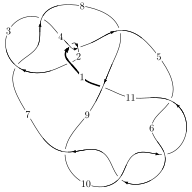
\includegraphics[width=112pt]{../../../GIT/diagram.site/Diagrams/png/286_11a_37.png}\\
\ \ \ A knot diagram\footnotemark}&
\allowdisplaybreaks
\textbf{Linearized knot diagam} \\
\cline{2-2}
 &
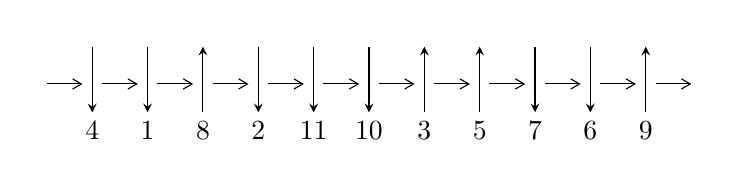
\begin{tikzpicture}[x=20pt, y=17pt]
	% nodes
	\node (C0) at (0, 0) {};
	\node (C1) at (1, 0) {};
	\node (C1U) at (1, +1) {};
	\node (C1D) at (1, -1) {4};

	\node (C2) at (2, 0) {};
	\node (C2U) at (2, +1) {};
	\node (C2D) at (2, -1) {1};

	\node (C3) at (3, 0) {};
	\node (C3U) at (3, +1) {};
	\node (C3D) at (3, -1) {8};

	\node (C4) at (4, 0) {};
	\node (C4U) at (4, +1) {};
	\node (C4D) at (4, -1) {2};

	\node (C5) at (5, 0) {};
	\node (C5U) at (5, +1) {};
	\node (C5D) at (5, -1) {11};

	\node (C6) at (6, 0) {};
	\node (C6U) at (6, +1) {};
	\node (C6D) at (6, -1) {10};

	\node (C7) at (7, 0) {};
	\node (C7U) at (7, +1) {};
	\node (C7D) at (7, -1) {3};

	\node (C8) at (8, 0) {};
	\node (C8U) at (8, +1) {};
	\node (C8D) at (8, -1) {5};

	\node (C9) at (9, 0) {};
	\node (C9U) at (9, +1) {};
	\node (C9D) at (9, -1) {7};

	\node (C10) at (10, 0) {};
	\node (C10U) at (10, +1) {};
	\node (C10D) at (10, -1) {6};

	\node (C11) at (11, 0) {};
	\node (C11U) at (11, +1) {};
	\node (C11D) at (11, -1) {9};
	\node (C12) at (12, 0) {};

	% arrows
	\draw[->,>={angle 60}]
	(C0) edge (C1) (C1) edge (C2) (C2) edge (C3) (C3) edge (C4) (C4) edge (C5) (C5) edge (C6) (C6) edge (C7) (C7) edge (C8) (C8) edge (C9) (C9) edge (C10) (C10) edge (C11) (C11) edge (C12) ;	\draw[->,>=stealth]
	(C1U) edge (C1D) (C2U) edge (C2D) (C3D) edge (C3U) (C4U) edge (C4D) (C5U) edge (C5D) (C6U) edge (C6D) (C7D) edge (C7U) (C8D) edge (C8U) (C9U) edge (C9D) (C10U) edge (C10D) (C11D) edge (C11U) ;
	\end{tikzpicture} \\
\hhline{~~} \\& 
\textbf{Solving Sequence} \\ \cline{2-2} 
 &
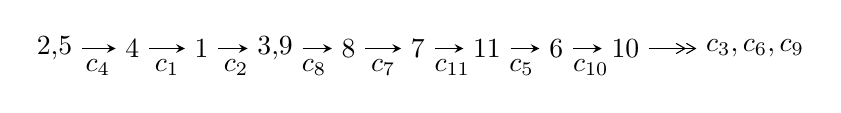
\begin{tikzpicture}[x=25pt, y=7pt]
	% node
	\node (A0) at (-1/8, 0) {2,5};
	\node (A1) at (1, 0) {4};
	\node (A2) at (2, 0) {1};
	\node (A3) at (49/16, 0) {3,9};
	\node (A4) at (33/8, 0) {8};
	\node (A5) at (41/8, 0) {7};
	\node (A6) at (49/8, 0) {11};
	\node (A7) at (57/8, 0) {6};
	\node (A8) at (65/8, 0) {10};
	\node (C1) at (1/2, -1) {$c_{4}$};
	\node (C2) at (3/2, -1) {$c_{1}$};
	\node (C3) at (5/2, -1) {$c_{2}$};
	\node (C4) at (29/8, -1) {$c_{8}$};
	\node (C5) at (37/8, -1) {$c_{7}$};
	\node (C6) at (45/8, -1) {$c_{11}$};
	\node (C7) at (53/8, -1) {$c_{5}$};
	\node (C8) at (61/8, -1) {$c_{10}$};
	\node (A9) at (10, 0) {$c_{3},c_{6},c_{9}$};

	% edge
	\draw[->,>=stealth]	
	(A0) edge (A1) (A1) edge (A2) (A2) edge (A3) (A3) edge (A4) (A4) edge (A5) (A5) edge (A6) (A6) edge (A7) (A7) edge (A8) ;
	\draw[->>,>={angle 60}]	
	(A8) edge (A9);
\end{tikzpicture} \\ 

\end{tabular} \\

\footnotetext{
The image of knot diagram is generated by the software ``\textbf{Draw programme}" developed by Andrew Bartholomew(\url{http://www.layer8.co.uk/maths/draw/index.htm\#Running-draw}), where we modified some parts for our purpose(\url{https://github.com/CATsTAILs/LinksPainter}).
}\phantom \\ \newline 
\centering \textbf{Ideals for irreducible components\footnotemark of $X_{\text{par}}$} 
 
\begin{align*}
I^u_{1}&=\langle 
-48 u^{49}+213 u^{48}+\cdots+4 b+63,\;29 u^{49}-118 u^{48}+\cdots+4 a-19,\;u^{50}-5 u^{49}+\cdots- u+1\rangle \\
I^u_{2}&=\langle 
b^4- b^3+b^2+1,\;a,\;u+1\rangle \\
\\
\end{align*}
\raggedright * 2 irreducible components of $\dim_{\mathbb{C}}=0$, with total 54 representations.\\
\footnotetext{All coefficients of polynomials are rational numbers. But the coefficients are sometimes approximated in decimal forms when there is not enough margin.}
\newpage
\renewcommand{\arraystretch}{1}
\centering \section*{I. $I^u_{1}= \langle -48 u^{49}+213 u^{48}+\cdots+4 b+63,\;29 u^{49}-118 u^{48}+\cdots+4 a-19,\;u^{50}-5 u^{49}+\cdots- u+1 \rangle$}
\flushleft \textbf{(i) Arc colorings}\\
\begin{tabular}{m{7pt} m{180pt} m{7pt} m{180pt} }
\flushright $a_{2}=$&$\begin{pmatrix}0\\u\end{pmatrix}$ \\
\flushright $a_{5}=$&$\begin{pmatrix}1\\0\end{pmatrix}$ \\
\flushright $a_{4}=$&$\begin{pmatrix}1\\- u^2\end{pmatrix}$ \\
\flushright $a_{1}=$&$\begin{pmatrix}u\\- u^3+u\end{pmatrix}$ \\
\flushright $a_{3}=$&$\begin{pmatrix}- u^3\\u^5- u^3+u\end{pmatrix}$ \\
\flushright $a_{9}=$&$\begin{pmatrix}-\frac{29}{4} u^{49}+\frac{59}{2} u^{48}+\cdots+\frac{5}{2} u+\frac{19}{4}\\12 u^{49}-\frac{213}{4} u^{48}+\cdots-\frac{1}{4} u-\frac{63}{4}\end{pmatrix}$ \\
\flushright $a_{8}=$&$\begin{pmatrix}-19.2500 u^{49}+82.7500 u^{48}+\cdots+2.75000 u+20.5000\\12 u^{49}-\frac{213}{4} u^{48}+\cdots-\frac{1}{4} u-\frac{63}{4}\end{pmatrix}$ \\
\flushright $a_{7}=$&$\begin{pmatrix}-9 u^{49}+\frac{149}{4} u^{48}+\cdots+\frac{17}{4} u+\frac{35}{4}\\\frac{51}{4} u^{49}-\frac{223}{4} u^{48}+\cdots+\frac{5}{4} u-15\end{pmatrix}$ \\
\flushright $a_{11}=$&$\begin{pmatrix}- u^{10}+3 u^8-2 u^7-4 u^6+4 u^5+u^4-4 u^3+u^2+2 u-1\\\frac{1}{8} u^{49}-\frac{1}{2} u^{48}+\cdots+2 u-\frac{1}{8}\end{pmatrix}$ \\
\flushright $a_{6}=$&$\begin{pmatrix}-\frac{1}{8} u^{49}+\frac{1}{2} u^{48}+\cdots-2 u+\frac{9}{8}\\\frac{21}{8} u^{49}-\frac{43}{4} u^{48}+\cdots-\frac{1}{4} u-\frac{23}{8}\end{pmatrix}$ \\
\flushright $a_{10}=$&$\begin{pmatrix}-\frac{1}{2} u^{49}+\frac{9}{4} u^{48}+\cdots+\frac{17}{4} u-\frac{1}{4}\\\frac{7}{2} u^{49}-17 u^{48}+\cdots-2 u-7\end{pmatrix}$\\ \flushright $a_{10}=$&$\begin{pmatrix}-\frac{1}{2} u^{49}+\frac{9}{4} u^{48}+\cdots+\frac{17}{4} u-\frac{1}{4}\\\frac{7}{2} u^{49}-17 u^{48}+\cdots-2 u-7\end{pmatrix}$\\&\end{tabular}
\flushleft \textbf{(ii) Obstruction class $= -1$}\\~\\
\flushleft \textbf{(iii) Cusp Shapes $= -\frac{85}{4} u^{49}+\frac{399}{4} u^{48}+\cdots-\frac{53}{4} u+\frac{65}{2}$}\\~\\
\newpage\renewcommand{\arraystretch}{1}
\flushleft \textbf{(iv) u-Polynomials at the component}\newline \\
\begin{tabular}{m{50pt}|m{274pt}}
Crossings & \hspace{64pt}u-Polynomials at each crossing \\
\hline $$\begin{aligned}c_{1},c_{4}\end{aligned}$$&$\begin{aligned}
&u^{50}-5 u^{49}+\cdots- u+1
\end{aligned}$\\
\hline $$\begin{aligned}c_{2}\end{aligned}$$&$\begin{aligned}
&u^{50}+23 u^{49}+\cdots-15 u+1
\end{aligned}$\\
\hline $$\begin{aligned}c_{3},c_{7}\end{aligned}$$&$\begin{aligned}
&u^{50}+u^{49}+\cdots+24 u+16
\end{aligned}$\\
\hline $$\begin{aligned}c_{5},c_{6},c_{9}\\c_{10}\end{aligned}$$&$\begin{aligned}
&u^{50}-2 u^{49}+\cdots-3 u+1
\end{aligned}$\\
\hline $$\begin{aligned}c_{8}\end{aligned}$$&$\begin{aligned}
&u^{50}-2 u^{49}+\cdots-1491 u+445
\end{aligned}$\\
\hline $$\begin{aligned}c_{11}\end{aligned}$$&$\begin{aligned}
&u^{50}+14 u^{49}+\cdots+1257 u+131
\end{aligned}$\\
\hline
\end{tabular}\\~\\
\newpage\renewcommand{\arraystretch}{1}
\flushleft \textbf{(v) Riley Polynomials at the component}\newline \\
\begin{tabular}{m{50pt}|m{274pt}}
Crossings & \hspace{64pt}Riley Polynomials at each crossing \\
\hline $$\begin{aligned}c_{1},c_{4}\end{aligned}$$&$\begin{aligned}
&y^{50}-23 y^{49}+\cdots+15 y+1
\end{aligned}$\\
\hline $$\begin{aligned}c_{2}\end{aligned}$$&$\begin{aligned}
&y^{50}+13 y^{49}+\cdots+3 y+1
\end{aligned}$\\
\hline $$\begin{aligned}c_{3},c_{7}\end{aligned}$$&$\begin{aligned}
&y^{50}-27 y^{49}+\cdots-2624 y+256
\end{aligned}$\\
\hline $$\begin{aligned}c_{5},c_{6},c_{9}\\c_{10}\end{aligned}$$&$\begin{aligned}
&y^{50}+58 y^{49}+\cdots+y+1
\end{aligned}$\\
\hline $$\begin{aligned}c_{8}\end{aligned}$$&$\begin{aligned}
&y^{50}-22 y^{49}+\cdots-648671 y+198025
\end{aligned}$\\
\hline $$\begin{aligned}c_{11}\end{aligned}$$&$\begin{aligned}
&y^{50}-10 y^{49}+\cdots+86009 y+17161
\end{aligned}$\\
\hline
\end{tabular}\\~\\
\newpage\flushleft \textbf{(vi) Complex Volumes and Cusp Shapes}
$$\begin{array}{c|c|c}  
\text{Solutions to }I^u_{1}& \I (\text{vol} + \sqrt{-1}CS) & \text{Cusp shape}\\
 \hline 
\begin{aligned}
u &= \phantom{-}0.582859 + 0.818130 I \\
a &= -0.981092 + 0.022618 I \\
b &= -1.038970 - 0.194067 I\end{aligned}
 & \phantom{-}5.74926 - 1.32005 I & \phantom{-}5.01799 + 3.45627 I \\ \hline\begin{aligned}
u &= \phantom{-}0.582859 - 0.818130 I \\
a &= -0.981092 - 0.022618 I \\
b &= -1.038970 + 0.194067 I\end{aligned}
 & \phantom{-}5.74926 + 1.32005 I & \phantom{-}5.01799 - 3.45627 I \\ \hline\begin{aligned}
u &= \phantom{-}0.435613 + 0.882797 I \\
a &= -1.36085 - 0.66520 I \\
b &= -1.36121 - 0.51636 I\end{aligned}
 & \phantom{-}4.77931 + 5.21174 I & \phantom{-}3.15504 - 5.31436 I \\ \hline\begin{aligned}
u &= \phantom{-}0.435613 - 0.882797 I \\
a &= -1.36085 + 0.66520 I \\
b &= -1.36121 + 0.51636 I\end{aligned}
 & \phantom{-}4.77931 - 5.21174 I & \phantom{-}3.15504 + 5.31436 I \\ \hline\begin{aligned}
u &= -0.928435 + 0.426925 I \\
a &= -1.46100 + 0.63623 I \\
b &= -0.719839 - 0.472231 I\end{aligned}
 & -1.61695 + 1.61236 I & -6.30739 - 1.92987 I \\ \hline\begin{aligned}
u &= -0.928435 - 0.426925 I \\
a &= -1.46100 - 0.63623 I \\
b &= -0.719839 + 0.472231 I\end{aligned}
 & -1.61695 - 1.61236 I & -6.30739 + 1.92987 I \\ \hline\begin{aligned}
u &= \phantom{-}0.429603 + 0.933534 I \\
a &= \phantom{-}1.62869 + 0.71121 I \\
b &= \phantom{-}1.52592 + 0.52069 I\end{aligned}
 & \phantom{-}12.7949 + 7.4878 I & \phantom{-}5.12788 - 3.72934 I \\ \hline\begin{aligned}
u &= \phantom{-}0.429603 - 0.933534 I \\
a &= \phantom{-}1.62869 - 0.71121 I \\
b &= \phantom{-}1.52592 - 0.52069 I\end{aligned}
 & \phantom{-}12.7949 - 7.4878 I & \phantom{-}5.12788 + 3.72934 I \\ \hline\begin{aligned}
u &= \phantom{-}0.935093 + 0.462361 I \\
a &= \phantom{-}0.633478 + 0.219321 I \\
b &= -0.112627 - 1.282310 I\end{aligned}
 & -1.42561 - 3.60776 I & -3.00000 + 7.46646 I \\ \hline\begin{aligned}
u &= \phantom{-}0.935093 - 0.462361 I \\
a &= \phantom{-}0.633478 - 0.219321 I \\
b &= -0.112627 + 1.282310 I\end{aligned}
 & -1.42561 + 3.60776 I & -3.00000 - 7.46646 I\\
 \hline 
 \end{array}$$\newpage$$\begin{array}{c|c|c}  
\text{Solutions to }I^u_{1}& \I (\text{vol} + \sqrt{-1}CS) & \text{Cusp shape}\\
 \hline 
\begin{aligned}
u &= \phantom{-}0.861919 + 0.408962 I \\
a &= -0.508762 - 0.083121 I \\
b &= \phantom{-}0.521608 + 1.221570 I\end{aligned}
 & -1.048050 + 0.087468 I & -1.42204 + 0.46193 I \\ \hline\begin{aligned}
u &= \phantom{-}0.861919 - 0.408962 I \\
a &= -0.508762 + 0.083121 I \\
b &= \phantom{-}0.521608 - 1.221570 I\end{aligned}
 & -1.048050 - 0.087468 I & -1.42204 - 0.46193 I \\ \hline\begin{aligned}
u &= \phantom{-}0.469477 + 0.811158 I \\
a &= \phantom{-}1.016760 + 0.499666 I \\
b &= \phantom{-}1.154940 + 0.462231 I\end{aligned}
 & \phantom{-}2.92925 + 1.64742 I & -0.497780 - 0.432754 I \\ \hline\begin{aligned}
u &= \phantom{-}0.469477 - 0.811158 I \\
a &= \phantom{-}1.016760 - 0.499666 I \\
b &= \phantom{-}1.154940 - 0.462231 I\end{aligned}
 & \phantom{-}2.92925 - 1.64742 I & -0.497780 + 0.432754 I \\ \hline\begin{aligned}
u &= \phantom{-}0.632917 + 0.878463 I \\
a &= \phantom{-}1.205340 - 0.345103 I \\
b &= \phantom{-}1.089650 - 0.054007 I\end{aligned}
 & \phantom{-}14.1472 - 2.8867 I & \phantom{-}6.24429 + 0. I\phantom{ +0.000000I} \\ \hline\begin{aligned}
u &= \phantom{-}0.632917 - 0.878463 I \\
a &= \phantom{-}1.205340 + 0.345103 I \\
b &= \phantom{-}1.089650 + 0.054007 I\end{aligned}
 & \phantom{-}14.1472 + 2.8867 I & \phantom{-}6.24429 + 0. I\phantom{ +0.000000I} \\ \hline\begin{aligned}
u &= -0.947722 + 0.527766 I \\
a &= \phantom{-}1.90433 - 0.66549 I \\
b &= \phantom{-}1.091640 + 0.560170 I\end{aligned}
 & -0.06909 + 4.84703 I & \phantom{-0.000000 } 0. - 7.27549 I \\ \hline\begin{aligned}
u &= -0.947722 - 0.527766 I \\
a &= \phantom{-}1.90433 + 0.66549 I \\
b &= \phantom{-}1.091640 - 0.560170 I\end{aligned}
 & -0.06909 - 4.84703 I & \phantom{-0.000000 -}0. + 7.27549 I \\ \hline\begin{aligned}
u &= -0.682129 + 0.592727 I \\
a &= -1.61933 + 1.77257 I \\
b &= -1.041110 + 0.419266 I\end{aligned}
 & \phantom{-}8.58536 - 2.27131 I & \phantom{-}2.70256 + 0. I\phantom{ +0.000000I} \\ \hline\begin{aligned}
u &= -0.682129 - 0.592727 I \\
a &= -1.61933 - 1.77257 I \\
b &= -1.041110 - 0.419266 I\end{aligned}
 & \phantom{-}8.58536 + 2.27131 I & \phantom{-}2.70256 + 0. I\phantom{ +0.000000I}\\
 \hline 
 \end{array}$$\newpage$$\begin{array}{c|c|c}  
\text{Solutions to }I^u_{1}& \I (\text{vol} + \sqrt{-1}CS) & \text{Cusp shape}\\
 \hline 
\begin{aligned}
u &= -0.957660 + 0.583300 I \\
a &= -2.17619 + 0.70245 I \\
b &= -1.33546 - 0.59049 I\end{aligned}
 & \phantom{-}7.74509 + 6.95904 I & \phantom{-0.000000 } 0 \\ \hline\begin{aligned}
u &= -0.957660 - 0.583300 I \\
a &= -2.17619 - 0.70245 I \\
b &= -1.33546 + 0.59049 I\end{aligned}
 & \phantom{-}7.74509 - 6.95904 I & \phantom{-0.000000 } 0 \\ \hline\begin{aligned}
u &= -1.123510 + 0.157529 I \\
a &= -0.550330 - 0.046161 I \\
b &= \phantom{-}0.309772 - 0.513002 I\end{aligned}
 & -2.34402 + 0.36505 I & \phantom{-0.000000 } 0 \\ \hline\begin{aligned}
u &= -1.123510 - 0.157529 I \\
a &= -0.550330 + 0.046161 I \\
b &= \phantom{-}0.309772 + 0.513002 I\end{aligned}
 & -2.34402 - 0.36505 I & \phantom{-0.000000 } 0 \\ \hline\begin{aligned}
u &= \phantom{-}0.803708 + 0.317036 I \\
a &= \phantom{-}0.479992 - 0.047063 I \\
b &= -0.96186 - 1.16924 I\end{aligned}
 & \phantom{-}5.81553 + 2.38249 I & \phantom{-}3.49858 + 1.94330 I \\ \hline\begin{aligned}
u &= \phantom{-}0.803708 - 0.317036 I \\
a &= \phantom{-}0.479992 + 0.047063 I \\
b &= -0.96186 + 1.16924 I\end{aligned}
 & \phantom{-}5.81553 - 2.38249 I & \phantom{-}3.49858 - 1.94330 I \\ \hline\begin{aligned}
u &= \phantom{-}1.027460 + 0.497180 I \\
a &= -0.894781 - 0.329352 I \\
b &= -0.41118 + 1.40760 I\end{aligned}
 & \phantom{-}4.51917 - 5.78869 I & \phantom{-0.000000 } 0 \\ \hline\begin{aligned}
u &= \phantom{-}1.027460 - 0.497180 I \\
a &= -0.894781 + 0.329352 I \\
b &= -0.41118 - 1.40760 I\end{aligned}
 & \phantom{-}4.51917 + 5.78869 I & \phantom{-0.000000 } 0 \\ \hline\begin{aligned}
u &= -0.701181 + 0.467599 I \\
a &= \phantom{-}1.30386 - 1.46602 I \\
b &= \phantom{-}0.748263 - 0.194492 I\end{aligned}
 & \phantom{-}0.729964 - 0.675494 I & \phantom{-}1.06714 + 1.67748 I \\ \hline\begin{aligned}
u &= -0.701181 - 0.467599 I \\
a &= \phantom{-}1.30386 + 1.46602 I \\
b &= \phantom{-}0.748263 + 0.194492 I\end{aligned}
 & \phantom{-}0.729964 + 0.675494 I & \phantom{-}1.06714 - 1.67748 I\\
 \hline 
 \end{array}$$\newpage$$\begin{array}{c|c|c}  
\text{Solutions to }I^u_{1}& \I (\text{vol} + \sqrt{-1}CS) & \text{Cusp shape}\\
 \hline 
\begin{aligned}
u &= -1.131350 + 0.330216 I \\
a &= \phantom{-}1.100770 + 0.196944 I \\
b &= \phantom{-}0.101239 + 1.026310 I\end{aligned}
 & \phantom{-}3.45731 + 1.19827 I & \phantom{-0.000000 } 0 \\ \hline\begin{aligned}
u &= -1.131350 - 0.330216 I \\
a &= \phantom{-}1.100770 - 0.196944 I \\
b &= \phantom{-}0.101239 - 1.026310 I\end{aligned}
 & \phantom{-}3.45731 - 1.19827 I & \phantom{-0.000000 } 0 \\ \hline\begin{aligned}
u &= \phantom{-}1.036300 + 0.664231 I \\
a &= -0.840415 - 1.006820 I \\
b &= -0.822961 + 0.495838 I\end{aligned}
 & \phantom{-}4.37658 - 4.22003 I & \phantom{-0.000000 } 0 \\ \hline\begin{aligned}
u &= \phantom{-}1.036300 - 0.664231 I \\
a &= -0.840415 + 1.006820 I \\
b &= -0.822961 - 0.495838 I\end{aligned}
 & \phantom{-}4.37658 + 4.22003 I & \phantom{-0.000000 } 0 \\ \hline\begin{aligned}
u &= -1.251000 + 0.108910 I \\
a &= \phantom{-}0.284422 + 0.232631 I \\
b &= -0.871117 + 0.511779 I\end{aligned}
 & -1.11589 - 2.48404 I & \phantom{-0.000000 } 0 \\ \hline\begin{aligned}
u &= -1.251000 - 0.108910 I \\
a &= \phantom{-}0.284422 - 0.232631 I \\
b &= -0.871117 - 0.511779 I\end{aligned}
 & -1.11589 + 2.48404 I & \phantom{-0.000000 } 0 \\ \hline\begin{aligned}
u &= \phantom{-}1.028110 + 0.728538 I \\
a &= \phantom{-}0.69726 + 1.30827 I \\
b &= \phantom{-}0.829533 - 0.089406 I\end{aligned}
 & \phantom{-}12.94610 - 3.03404 I & \phantom{-0.000000 } 0 \\ \hline\begin{aligned}
u &= \phantom{-}1.028110 - 0.728538 I \\
a &= \phantom{-}0.69726 - 1.30827 I \\
b &= \phantom{-}0.829533 + 0.089406 I\end{aligned}
 & \phantom{-}12.94610 + 3.03404 I & \phantom{-0.000000 } 0 \\ \hline\begin{aligned}
u &= \phantom{-}1.100010 + 0.633178 I \\
a &= \phantom{-}1.17840 + 0.90974 I \\
b &= \phantom{-}1.17520 - 0.79670 I\end{aligned}
 & \phantom{-}1.03930 - 7.06574 I & \phantom{-0.000000 } 0 \\ \hline\begin{aligned}
u &= \phantom{-}1.100010 - 0.633178 I \\
a &= \phantom{-}1.17840 - 0.90974 I \\
b &= \phantom{-}1.17520 + 0.79670 I\end{aligned}
 & \phantom{-}1.03930 + 7.06574 I & \phantom{-0.000000 } 0\\
 \hline 
 \end{array}$$\newpage$$\begin{array}{c|c|c}  
\text{Solutions to }I^u_{1}& \I (\text{vol} + \sqrt{-1}CS) & \text{Cusp shape}\\
 \hline 
\begin{aligned}
u &= \phantom{-}1.133290 + 0.650060 I \\
a &= -1.34813 - 1.01237 I \\
b &= -1.43569 + 0.74867 I\end{aligned}
 & \phantom{-}2.67414 - 10.86920 I & \phantom{-0.000000 } 0 \\ \hline\begin{aligned}
u &= \phantom{-}1.133290 - 0.650060 I \\
a &= -1.34813 + 1.01237 I \\
b &= -1.43569 - 0.74867 I\end{aligned}
 & \phantom{-}2.67414 + 10.86920 I & \phantom{-0.000000 } 0 \\ \hline\begin{aligned}
u &= -1.311520 + 0.106975 I \\
a &= -0.125488 - 0.322812 I \\
b &= \phantom{-}1.176990 - 0.583698 I\end{aligned}
 & \phantom{-}6.58516 - 4.39707 I & \phantom{-0.000000 } 0 \\ \hline\begin{aligned}
u &= -1.311520 - 0.106975 I \\
a &= -0.125488 + 0.322812 I \\
b &= \phantom{-}1.176990 + 0.583698 I\end{aligned}
 & \phantom{-}6.58516 + 4.39707 I & \phantom{-0.000000 } 0 \\ \hline\begin{aligned}
u &= \phantom{-}1.154930 + 0.665889 I \\
a &= \phantom{-}1.46673 + 1.10969 I \\
b &= \phantom{-}1.62351 - 0.67827 I\end{aligned}
 & \phantom{-}10.5867 - 13.3384 I & \phantom{-0.000000 } 0 \\ \hline\begin{aligned}
u &= \phantom{-}1.154930 - 0.665889 I \\
a &= \phantom{-}1.46673 - 1.10969 I \\
b &= \phantom{-}1.62351 + 0.67827 I\end{aligned}
 & \phantom{-}10.5867 + 13.3384 I & \phantom{-0.000000 } 0 \\ \hline\begin{aligned}
u &= \phantom{-}0.004533 + 0.531412 I \\
a &= \phantom{-}0.34509 - 1.83693 I \\
b &= -0.385670 - 0.859631 I\end{aligned}
 & \phantom{-}6.72549 + 2.13344 I & \phantom{-}2.98920 - 3.27411 I \\ \hline\begin{aligned}
u &= \phantom{-}0.004533 - 0.531412 I \\
a &= \phantom{-}0.34509 + 1.83693 I \\
b &= -0.385670 + 0.859631 I\end{aligned}
 & \phantom{-}6.72549 - 2.13344 I & \phantom{-}2.98920 + 3.27411 I \\ \hline\begin{aligned}
u &= -0.101318 + 0.238648 I \\
a &= -0.87875 + 2.12555 I \\
b &= \phantom{-}0.149430 + 0.468790 I\end{aligned}
 & -0.000511 + 1.051120 I & -0.14079 - 6.76805 I \\ \hline\begin{aligned}
u &= -0.101318 - 0.238648 I \\
a &= -0.87875 - 2.12555 I \\
b &= \phantom{-}0.149430 - 0.468790 I\end{aligned}
 & -0.000511 - 1.051120 I & -0.14079 + 6.76805 I\\
 \hline 
 \end{array}$$\newpage\newpage\renewcommand{\arraystretch}{1}
\centering \section*{II. $I^u_{2}= \langle b^4- b^3+b^2+1,\;a,\;u+1 \rangle$}
\flushleft \textbf{(i) Arc colorings}\\
\begin{tabular}{m{7pt} m{180pt} m{7pt} m{180pt} }
\flushright $a_{2}=$&$\begin{pmatrix}0\\-1\end{pmatrix}$ \\
\flushright $a_{5}=$&$\begin{pmatrix}1\\0\end{pmatrix}$ \\
\flushright $a_{4}=$&$\begin{pmatrix}1\\-1\end{pmatrix}$ \\
\flushright $a_{1}=$&$\begin{pmatrix}-1\\0\end{pmatrix}$ \\
\flushright $a_{3}=$&$\begin{pmatrix}1\\-1\end{pmatrix}$ \\
\flushright $a_{9}=$&$\begin{pmatrix}0\\b\end{pmatrix}$ \\
\flushright $a_{8}=$&$\begin{pmatrix}- b\\b\end{pmatrix}$ \\
\flushright $a_{7}=$&$\begin{pmatrix}- b\\b\end{pmatrix}$ \\
\flushright $a_{11}=$&$\begin{pmatrix}-1\\- b^2\end{pmatrix}$ \\
\flushright $a_{6}=$&$\begin{pmatrix}b^2+1\\b^3- b^2-1\end{pmatrix}$ \\
\flushright $a_{10}=$&$\begin{pmatrix}- b^3\\b^3+b\end{pmatrix}$\\ \flushright $a_{10}=$&$\begin{pmatrix}- b^3\\b^3+b\end{pmatrix}$\\&\end{tabular}
\flushleft \textbf{(ii) Obstruction class $= 1$}\\~\\
\flushleft \textbf{(iii) Cusp Shapes $= -4 b^2+3 b-5$}\\~\\
\newpage\renewcommand{\arraystretch}{1}
\flushleft \textbf{(iv) u-Polynomials at the component}\newline \\
\begin{tabular}{m{50pt}|m{274pt}}
Crossings & \hspace{64pt}u-Polynomials at each crossing \\
\hline $$\begin{aligned}c_{1}\end{aligned}$$&$\begin{aligned}
&(u-1)^4
\end{aligned}$\\
\hline $$\begin{aligned}c_{2},c_{4}\end{aligned}$$&$\begin{aligned}
&(u+1)^4
\end{aligned}$\\
\hline $$\begin{aligned}c_{3},c_{7}\end{aligned}$$&$\begin{aligned}
&u^4
\end{aligned}$\\
\hline $$\begin{aligned}c_{5},c_{6}\end{aligned}$$&$\begin{aligned}
&u^4- u^3+3 u^2-2 u+1
\end{aligned}$\\
\hline $$\begin{aligned}c_{8},c_{11}\end{aligned}$$&$\begin{aligned}
&u^4+u^3+u^2+1
\end{aligned}$\\
\hline $$\begin{aligned}c_{9},c_{10}\end{aligned}$$&$\begin{aligned}
&u^4+u^3+3 u^2+2 u+1
\end{aligned}$\\
\hline
\end{tabular}\\~\\
\newpage\renewcommand{\arraystretch}{1}
\flushleft \textbf{(v) Riley Polynomials at the component}\newline \\
\begin{tabular}{m{50pt}|m{274pt}}
Crossings & \hspace{64pt}Riley Polynomials at each crossing \\
\hline $$\begin{aligned}c_{1},c_{2},c_{4}\end{aligned}$$&$\begin{aligned}
&(y-1)^4
\end{aligned}$\\
\hline $$\begin{aligned}c_{3},c_{7}\end{aligned}$$&$\begin{aligned}
&y^4
\end{aligned}$\\
\hline $$\begin{aligned}c_{5},c_{6},c_{9}\\c_{10}\end{aligned}$$&$\begin{aligned}
&y^4+5 y^3+7 y^2+2 y+1
\end{aligned}$\\
\hline $$\begin{aligned}c_{8},c_{11}\end{aligned}$$&$\begin{aligned}
&y^4+y^3+3 y^2+2 y+1
\end{aligned}$\\
\hline
\end{tabular}\\~\\
\newpage\flushleft \textbf{(vi) Complex Volumes and Cusp Shapes}
$$\begin{array}{c|c|c}  
\text{Solutions to }I^u_{2}& \I (\text{vol} + \sqrt{-1}CS) & \text{Cusp shape}\\
 \hline 
\begin{aligned}
u &= -1.00000\phantom{ +0.000000I} \\
a &= \phantom{-0.000000 } 0 \\
b &= -0.351808 + 0.720342 I\end{aligned}
 & -1.85594 - 1.41510 I & -4.47493 + 4.18840 I \\ \hline\begin{aligned}
u &= -1.00000\phantom{ +0.000000I} \\
a &= \phantom{-0.000000 } 0 \\
b &= -0.351808 - 0.720342 I\end{aligned}
 & -1.85594 + 1.41510 I & -4.47493 - 4.18840 I \\ \hline\begin{aligned}
u &= -1.00000\phantom{ +0.000000I} \\
a &= \phantom{-0.000000 } 0 \\
b &= \phantom{-}0.851808 + 0.911292 I\end{aligned}
 & \phantom{-}5.14581 + 3.16396 I & -2.02507 - 3.47609 I \\ \hline\begin{aligned}
u &= -1.00000\phantom{ +0.000000I} \\
a &= \phantom{-0.000000 } 0 \\
b &= \phantom{-}0.851808 - 0.911292 I\end{aligned}
 & \phantom{-}5.14581 - 3.16396 I & -2.02507 + 3.47609 I\\
 \hline 
 \end{array}$$\newpage
\newpage\renewcommand{\arraystretch}{1}
\centering \section*{ III. u-Polynomials}
\begin{tabular}{m{50pt}|m{274pt}}
Crossings & \hspace{64pt}u-Polynomials at each crossing \\
\hline $$\begin{aligned}c_{1}\end{aligned}$$&$\begin{aligned}
&((u-1)^4)(u^{50}-5 u^{49}+\cdots- u+1)
\end{aligned}$\\
\hline $$\begin{aligned}c_{2}\end{aligned}$$&$\begin{aligned}
&((u+1)^4)(u^{50}+23 u^{49}+\cdots-15 u+1)
\end{aligned}$\\
\hline $$\begin{aligned}c_{3},c_{7}\end{aligned}$$&$\begin{aligned}
&u^4(u^{50}+u^{49}+\cdots+24 u+16)
\end{aligned}$\\
\hline $$\begin{aligned}c_{4}\end{aligned}$$&$\begin{aligned}
&((u+1)^4)(u^{50}-5 u^{49}+\cdots- u+1)
\end{aligned}$\\
\hline $$\begin{aligned}c_{5},c_{6}\end{aligned}$$&$\begin{aligned}
&(u^4- u^3+3 u^2-2 u+1)(u^{50}-2 u^{49}+\cdots-3 u+1)
\end{aligned}$\\
\hline $$\begin{aligned}c_{8}\end{aligned}$$&$\begin{aligned}
&(u^4+u^3+u^2+1)(u^{50}-2 u^{49}+\cdots-1491 u+445)
\end{aligned}$\\
\hline $$\begin{aligned}c_{9},c_{10}\end{aligned}$$&$\begin{aligned}
&(u^4+u^3+3 u^2+2 u+1)(u^{50}-2 u^{49}+\cdots-3 u+1)
\end{aligned}$\\
\hline $$\begin{aligned}c_{11}\end{aligned}$$&$\begin{aligned}
&(u^4+u^3+u^2+1)(u^{50}+14 u^{49}+\cdots+1257 u+131)
\end{aligned}$\\
\hline
\end{tabular}\newpage\renewcommand{\arraystretch}{1}
\centering \section*{ IV. Riley Polynomials}
\begin{tabular}{m{50pt}|m{274pt}}
Crossings & \hspace{64pt}Riley Polynomials at each crossing \\
\hline $$\begin{aligned}c_{1},c_{4}\end{aligned}$$&$\begin{aligned}
&((y-1)^4)(y^{50}-23 y^{49}+\cdots+15 y+1)
\end{aligned}$\\
\hline $$\begin{aligned}c_{2}\end{aligned}$$&$\begin{aligned}
&((y-1)^4)(y^{50}+13 y^{49}+\cdots+3 y+1)
\end{aligned}$\\
\hline $$\begin{aligned}c_{3},c_{7}\end{aligned}$$&$\begin{aligned}
&y^4(y^{50}-27 y^{49}+\cdots-2624 y+256)
\end{aligned}$\\
\hline $$\begin{aligned}c_{5},c_{6},c_{9}\\c_{10}\end{aligned}$$&$\begin{aligned}
&(y^4+5 y^3+7 y^2+2 y+1)(y^{50}+58 y^{49}+\cdots+y+1)
\end{aligned}$\\
\hline $$\begin{aligned}c_{8}\end{aligned}$$&$\begin{aligned}
&(y^4+y^3+3 y^2+2 y+1)(y^{50}-22 y^{49}+\cdots-648671 y+198025)
\end{aligned}$\\
\hline $$\begin{aligned}c_{11}\end{aligned}$$&$\begin{aligned}
&(y^4+y^3+3 y^2+2 y+1)(y^{50}-10 y^{49}+\cdots+86009 y+17161)
\end{aligned}$\\
\hline
\end{tabular}
\vskip 2pc
\end{document}